\documentclass[../Tesi.tex]{subfiles}
\begin{document}

\chapter{Studi svolti e Analisi dei Risultati}
Basandomi sui risultati descritti nell'articolo in esame \cite{DBLP:journals/corr/abs-2008-13589} e riportati nel precedente capitolo, ho tentato di rispondere ad alcune delle domande rimaste insolute.\\*
La mia attenzione \'e stata rivolta in particolare al tempo di assorbimento che si ottiene adottando Majority-Dynamics su alcune topologie quando il bias \'e inferiore a $\frac{1}{2}$.\\*
Le topologie analizzate sono state:
\begin{itemize}
\item Ipercubo
\item Clique
\item Ciclo
\item Modello di Erd{\"o}s R\'enyi G($n$,$p$) \cite{Erdos:1959:pmd}
\end{itemize}

\section{Cenni al software di simulazione}
Per ottenere e, successivamente, analizzare i tempi di assorbimento, ho sviluppato un software in grado di simulare i processi descritti nel modello preso in esame.
Di seguito \'e riportato lo pseudocodice di alcune delle funzioni principali utilizzate.\\*

\begin{algorithm}[H]
  \For{v $\in$ graph.vertices}{
    \If{v.opinion == 0}{
        \Return False\;
    }
  }
  \Return True\;
\caption{absorptionStateReached(\emph{graph}: GraphTool.Graph)}
\end{algorithm}
 
 \hfill \break
 
\begin{algorithm}[H]
  graph $\gets$ config.graph\;
  bias $\gets$ config.bias\;
  updateRule $\gets$ config.opinionUpdateRule\;
  rounds $\gets$ 0\;

  \While{$\neg$ absorptionStateReached(graph)}
  {
    v $\gets$ random.choice(graph.vertices)\;
    \eIf{random(0,1) $\leq$ bias}{
      v.opinion $\gets$ 1\;
    }{
        v.opinion $\gets$ updateRule.run(graph,v)\;
    }
    rounds $\gets$ rounds + 1\;
  }
  simulationResult $\gets$ \emph{new} SimulationResult(config, rounds)\;
  \Return simulationResult\;
\caption{runSimulationOn(\emph{config}: SimulationConfigurator)}
\end{algorithm}
 
\hfill \break

Notare come \emph{config.opinionUpdateRule} sia un oggetto ottenuto tramite un'interfaccia che permette di implementare la dinamica di aggiornamento preferita eseguendo un \emph{override} del metodo \emph{run}. Di seguito l'implementazione in pseudocodice di tale metodo per Majority-Dynamics.\\*

\begin{algorithm}[H]
  neighbors $\gets$ v.neighbors()\;
  \If{$\neg$ neighbors}{
    \Return v.opinion\;
  }
  counter0 $\gets$ 0\;
  counter1 $\gets$ 0\;
  
  \For{v $\in$ neighbors}{
    \If{v.opinion == 1}{
        counter1 $\gets$ counter1+1\;
    }
    \If{v.opinion == 0}{
        counter0 $\gets$ counter0+1\;
    }
  }
  
  \If{counter0 $>$ counter1}{
        \Return 0\;
  }
  \If{counter1 $>$ counter0}{
        \Return 1\;
  }
  \Return random.choice([0,1])\;
\caption{MajorityDynamics.run(\emph{graph}: GraphTool.Graph, \emph{v}: GraphTool.Vertex)}
\end{algorithm}

\section{Analisi di Clique, Ipercubo e Ciclo}
I primi test eseguiti sono serviti a verificare l'accuratezza del software e correggerne eventuali errori. Ogni test \'e composto da 100 simulazioni, configurate con Majority-Dynamics e bias pari a $\frac{1}{2}$.\\*
I test sono stati eseguiti su Ipercubi, Cliques e Cicli, in dimensioni che vanno da $2^{5^{\mathrm{}}}$ fino a $2^{12^{\mathrm{}}}$ vertici.\\*
\begin{figure}[H]
    \centering
    \includegraphics[width=0.8\linewidth]{imgs/Test/Test_05.png}
    \caption*{Test con $\alpha = \frac{1}{2}$}
\end{figure}
I risultati ottenuti sono perfettamente in linea con quanto dimostrato teoricamente in \emph{Biased Opinion Dynamics} \cite{DBLP:journals/corr/abs-2008-13589}. Per quanto riguarda il Ciclo, il tempo di assorbimento \'e stato pari a $O(\frac{1}{\alpha}n\log{}n)$. \\*
Riguardo Clique e Ipercubo, per i quali il grado minimo \'e pari a $\Omega(\log{}n)$, il tempo di assorbimento con bias pari a $\frac{1}{2}$ si \'e rivelato essere $O(n\log{}n)$, anche questa volta confermando quanto evidenziato nell'articolo \cite{DBLP:journals/corr/abs-2008-13589}.\\*
Una volta appurato che il software simulasse correttamente i processi descritti, ottenendo risultati conformi a quanto atteso, sono stati eseguiti test metodologicamente analoghi ai precedenti, adottando per\'o un bias verso l'opinione dominante pari a $\frac{1}{4}$, di fatto dimezzandolo.\\*
\begin{figure}[H]
    \centering
    \includegraphics[width=0.8\linewidth]{imgs/Test/Test_025.png}
    \caption*{Test con $\alpha = \frac{1}{4}$}
\end{figure}
Per quanto riguarda il Ciclo e la Clique, sono stati ancora una volta confermati i risultati attesi.
Lo stato di assorbimento per il Ciclo \'e stato nuovamente raggiunto in $O(\frac{1}{\alpha}n\log{}n)$ passi in valore atteso. Nello specifico, dimezzando il valore del bias, i tempi di assorbimento per tale topologia sono raddoppiati, suggerendo una proporzionalit\'a inversa tra il tempo di assorbimento e il valore del bias.\\*
D'altra parte, come previsto, \'e stato impossibile ultimare i test per la Clique, in quanto, con un bias inferiore a $\frac{1}{2}$, il numero di passi necessari a raggiungere lo stato di assorbimento \'e diventato esponenziale nel grado minimo ($n-1$ per le Clique), di fatto rendendo impossibile lo svolgimento dei test gi\'a dalla dimensione di $2^{6^{\mathrm{}}}$.\\*
L'articolo in esame \cite{DBLP:journals/corr/abs-2008-13589} lascia aperta la domanda inerente al comportamento dell'Ipercubo con un bias cos\'i basso. Dai risultati dei test si evince come l'Ipercubo abbia un comportamento assimilabile a quello del Ciclo, raggiungendo perci\'o lo stato di assorbimento in $O(n\log{}n)$ passi.
\section{Analisi del Modello di Erd{\"o}s R\'enyi}
Questa sezione \'e dedicata all'analisi dei tempi di assorbimento per topologie non regolari, cio\'e grafi per i quali i vertici non condividono lo stesso grado.\\
Tali topologie sono state generate scrivendo un algoritmo aleatorio basato sul Modello di Erd{\"o}s R\'enyi G($n$,$p$) \cite{Erdos:1959:pmd}.\\*
In tale modello, dato un grafo G($V$,$E$) con $|V|$ = $n$,
\begin{equation}
    \forall \: u,v \in V,\; P((u,v) \in E)=p.
\end{equation}
I test eseguiti sono composti da 100 simulazioni, configurate con Majority-Dynamics e bias pari a $\frac{1}{4}$.\\*
Le topologie prese in considerazione hanno dimensioni che vanno da $2^{5^{\mathrm{}}}$ fino a $2^{12^{\mathrm{}}}$ vertici e sono state generate con il modello G($n$,$p$) descritto precedentemente, utilizzando i seguenti valori di $p$:
\begin{itemize}
\item $p$ = $\frac{1-\epsilon}{n}$ con $\epsilon=\frac{1}{2}$, per il quale il grafo risulta principalmente sparso, con alta probabilit\'a (in tabella indicato come ER\_SP).
\item $p$ = $\frac{1+\epsilon}{n}$ con $\epsilon=\frac{1}{2}$, per il quale il grafo presenta una \emph{giant component} circondata da componenti pi\'u piccole di dimensione $O(\log{}n)$, con alta probabilit\'a (in tabella indicato come ER\_GC).
\item $p$ = $\frac{\log{}n}{n}$, per il quale il grafo risulta connesso e discretamente denso, con alta probabilit\'a (in tabella indicato come ER\_DN).
\end{itemize}
\begin{figure}[H]
\centering
    \begin{subfigure}{0.3\textwidth}
      \centering
      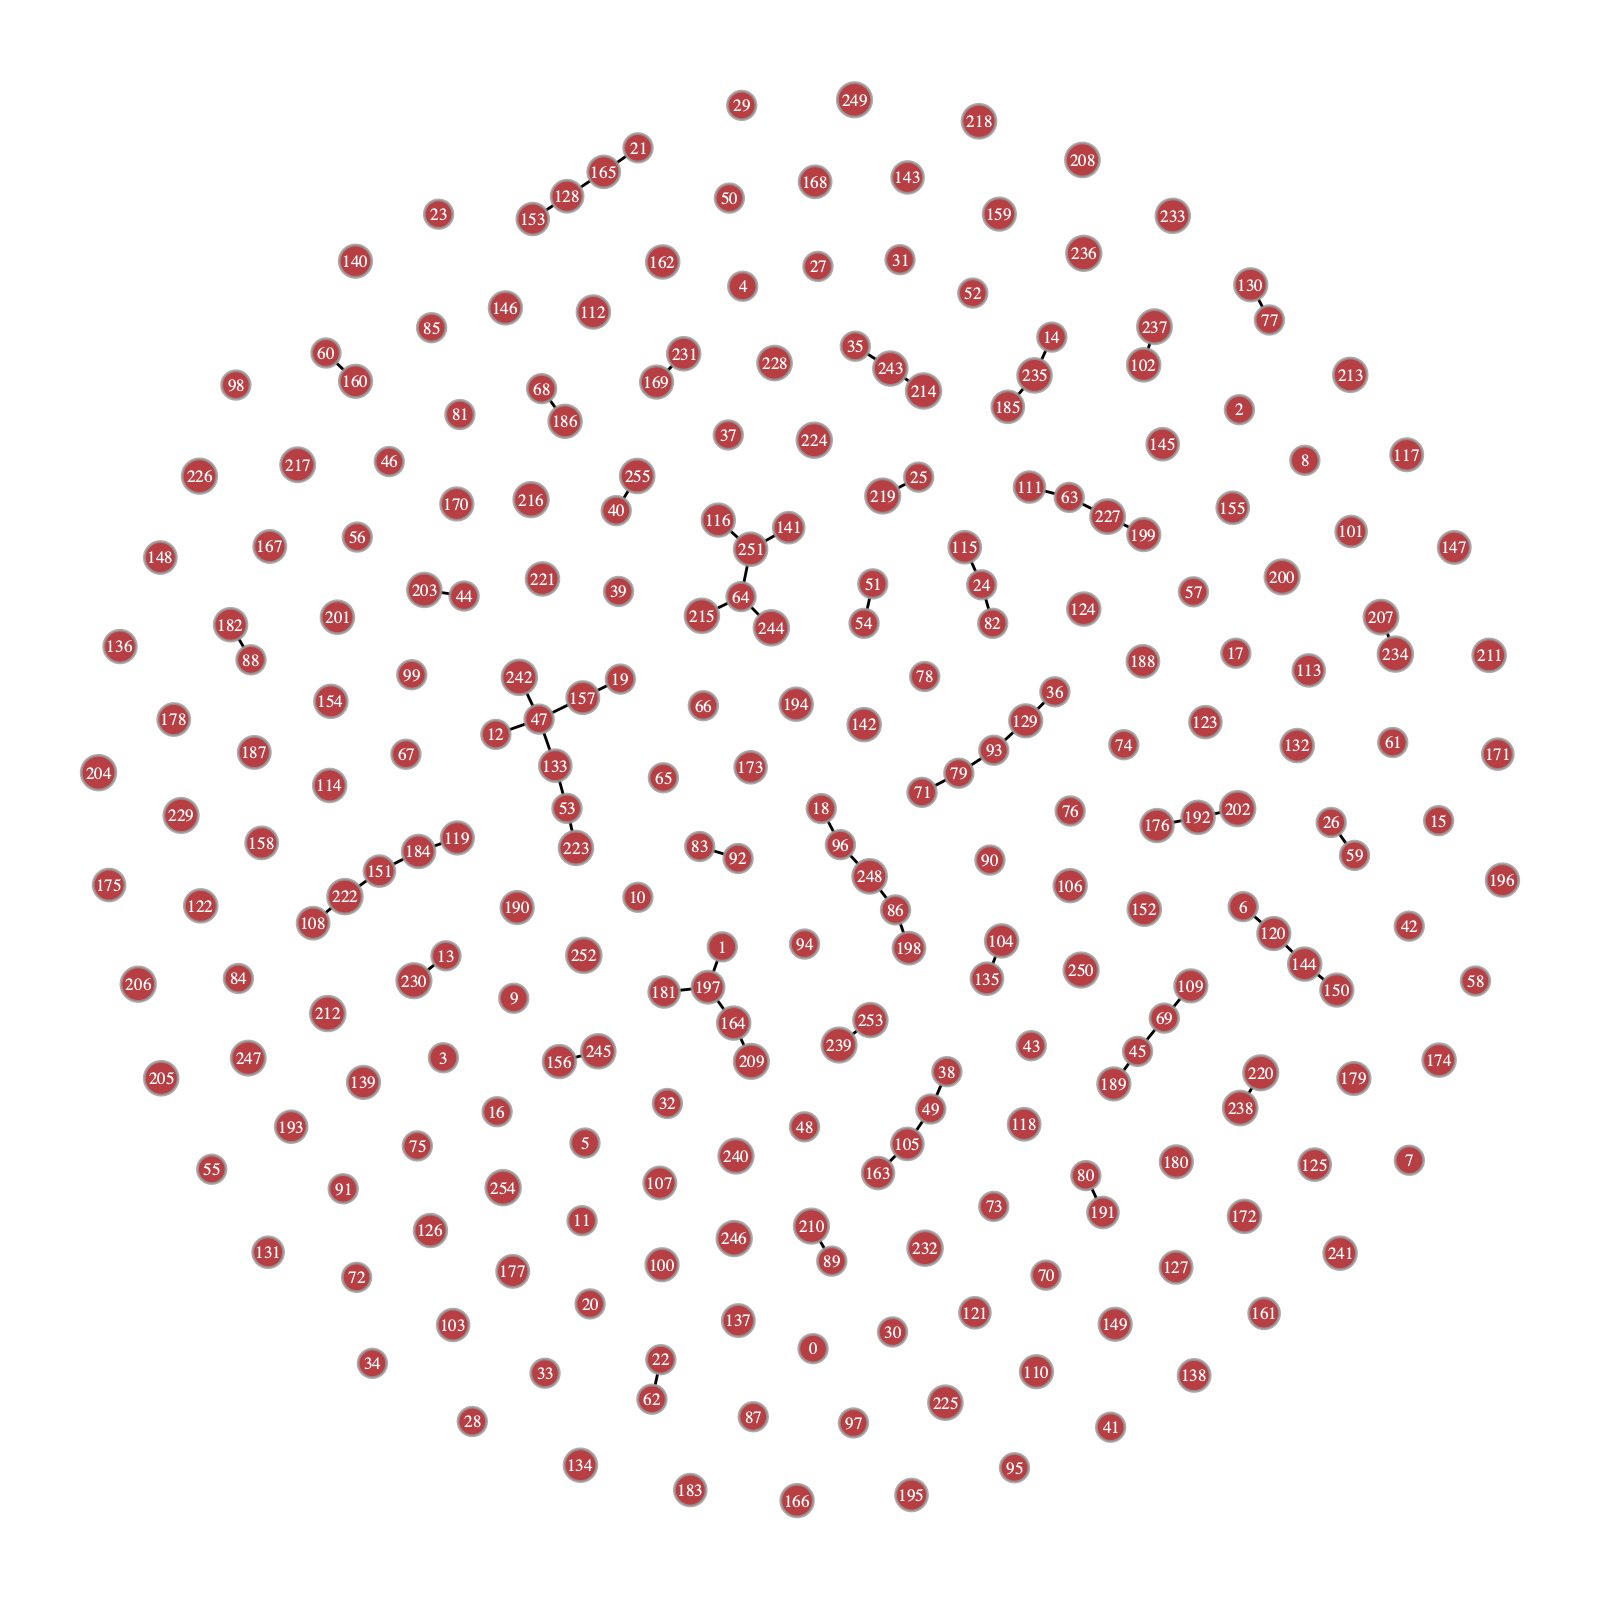
\includegraphics[width=0.6\linewidth]{imgs/ER_Examples/ER_SP.png}
      \caption{}
      \label{fig:sub1}
    \end{subfigure}%
    \begin{subfigure}{0.3\textwidth}
      \centering
      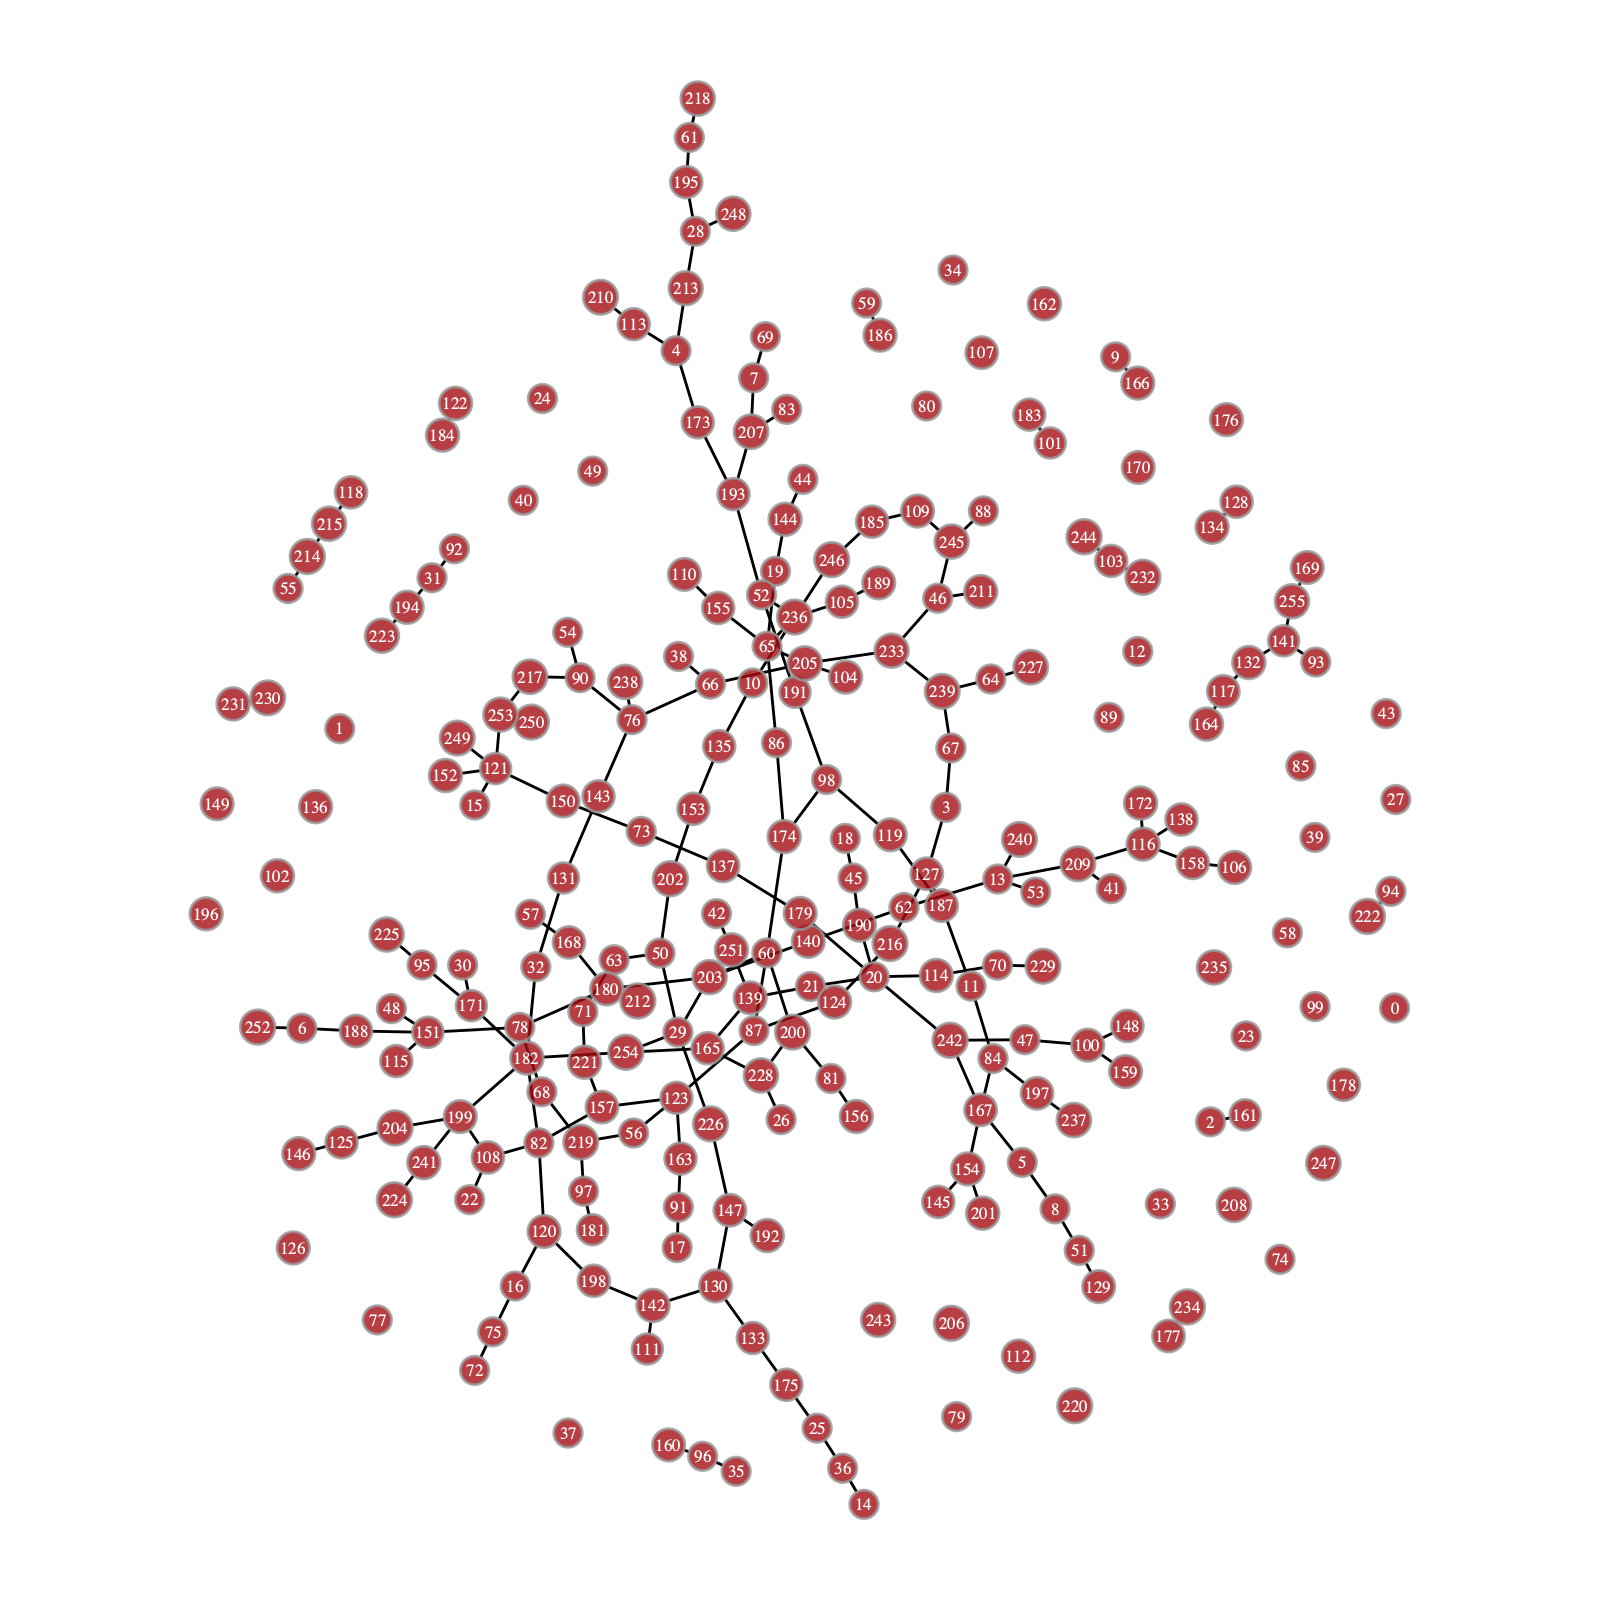
\includegraphics[width=0.6\linewidth]{imgs/ER_Examples/ER_GC.png}
      \caption{}
      \label{fig:sub2}
    \end{subfigure}
    \begin{subfigure}{0.3\textwidth}
      \centering
      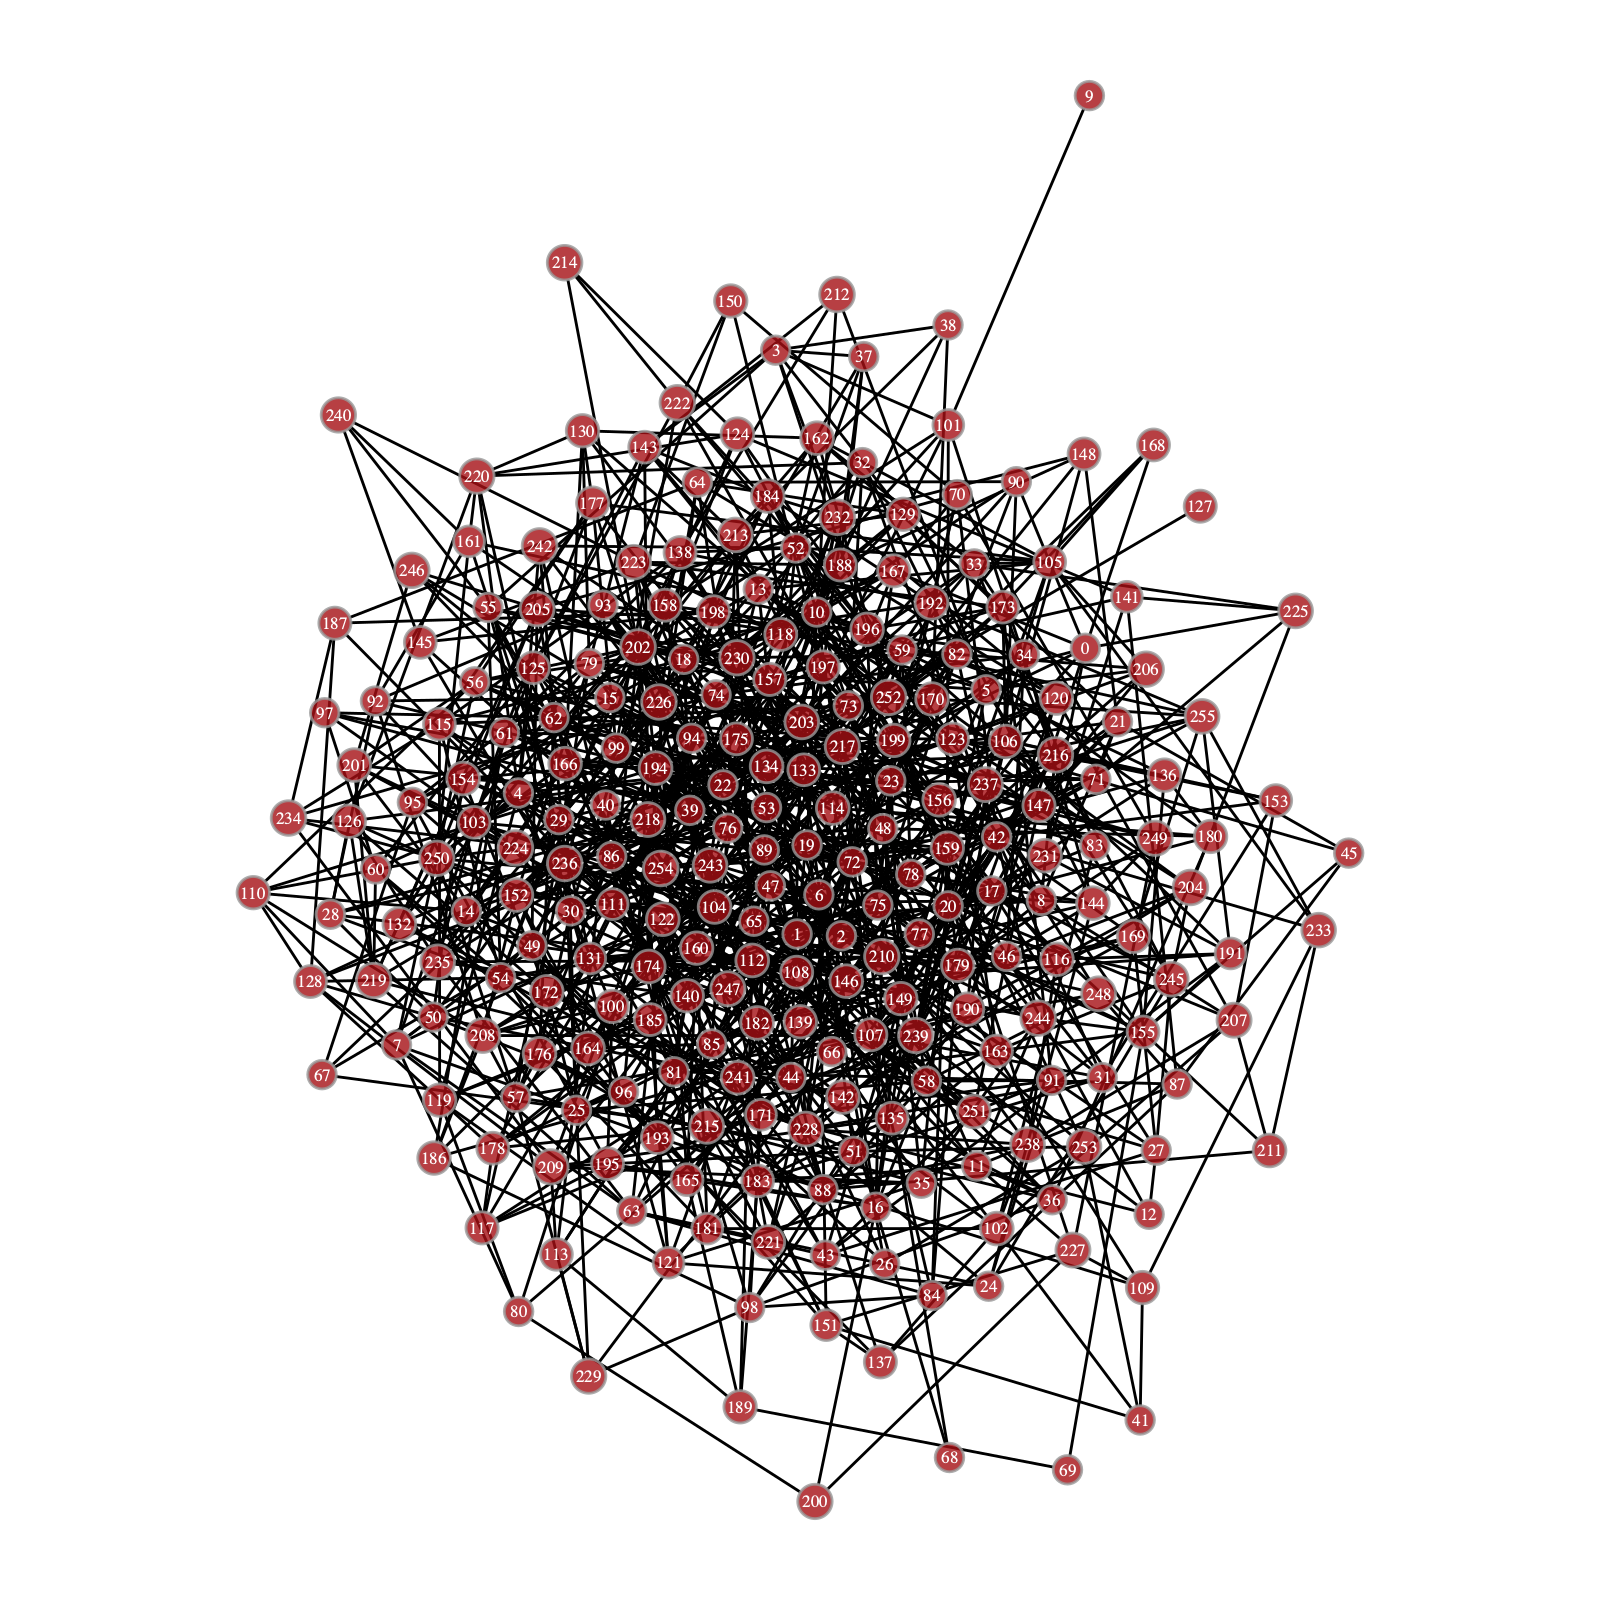
\includegraphics[width=0.6\linewidth]{imgs/ER_Examples/ER_DN.png}
      \caption{}
      \label{fig:sub1}
    \end{subfigure}%
\caption*{Esempi ottenuti utilizzando le probabilit\'a descritte. $n$=256, $\epsilon$=$\frac{1}{2}$}
\end{figure}
\begin{figure}[H]
    \centering
    \includegraphics[width=0.8\linewidth]{imgs/Test/Test_ER.png}
    \caption*{Test Erd{\"o}s R\'enyi con $\alpha = \frac{1}{4}$}
\end{figure}
I risultati dei test descrivono un andamento meno prevedibile di quanto ci si potesse aspettare.\\*
Per valori di $p$ che si allontanano dallo 0 il tempo di assorbimento inizia a diminuire, mentre gli studi compiuti sulla Clique \cite{DBLP:journals/corr/abs-2008-13589} evidenziano una crescita esponenziale nel grado minimo quando $p$ tende a 1. La curva che si ottiene perci\'o fissando $n$ e facendo variare $p$ non risulta essere monotona crescente, in contrasto con quanto atteso.\\*
Per indagare tale comportamento in modo pi\'u approfondito, ho eseguito ulteriori test con la seguente configurazione:
\begin{itemize}
    \item $n=512$ e $n=1024$
    \item $\alpha=\frac{1}{4}$
    \item $p$ assume valori in [ $\frac{1-\epsilon}{n}$ , $\frac{{(1+\epsilon)}\log{}n}{n}$ ] t.c. $p_{i+1}$ - $p_{i}$ = 0.001
\end{itemize}
Di seguito sono mostrati due grafici ottenuti eseguendo i test sopracitati.\\*
\begin{figure}[H]
\centering
    \begin{subfigure}[b]{0.45\textwidth}
      \centering
      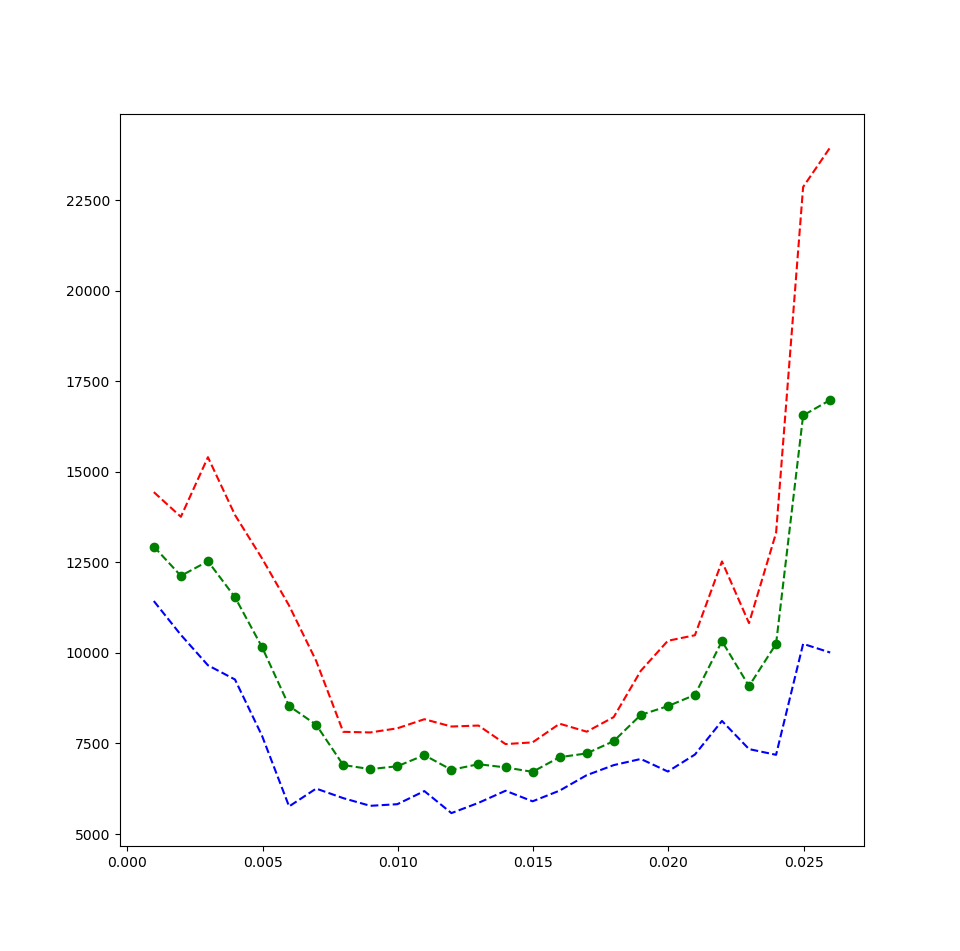
\includegraphics[width=0.8\linewidth]{imgs/ER_p_variation/n=512 a=025.png}
      \caption*{$n=512$}
      \label{fig:sub1}
    \end{subfigure}%
    \begin{subfigure}[b]{0.45\textwidth}
      \centering
      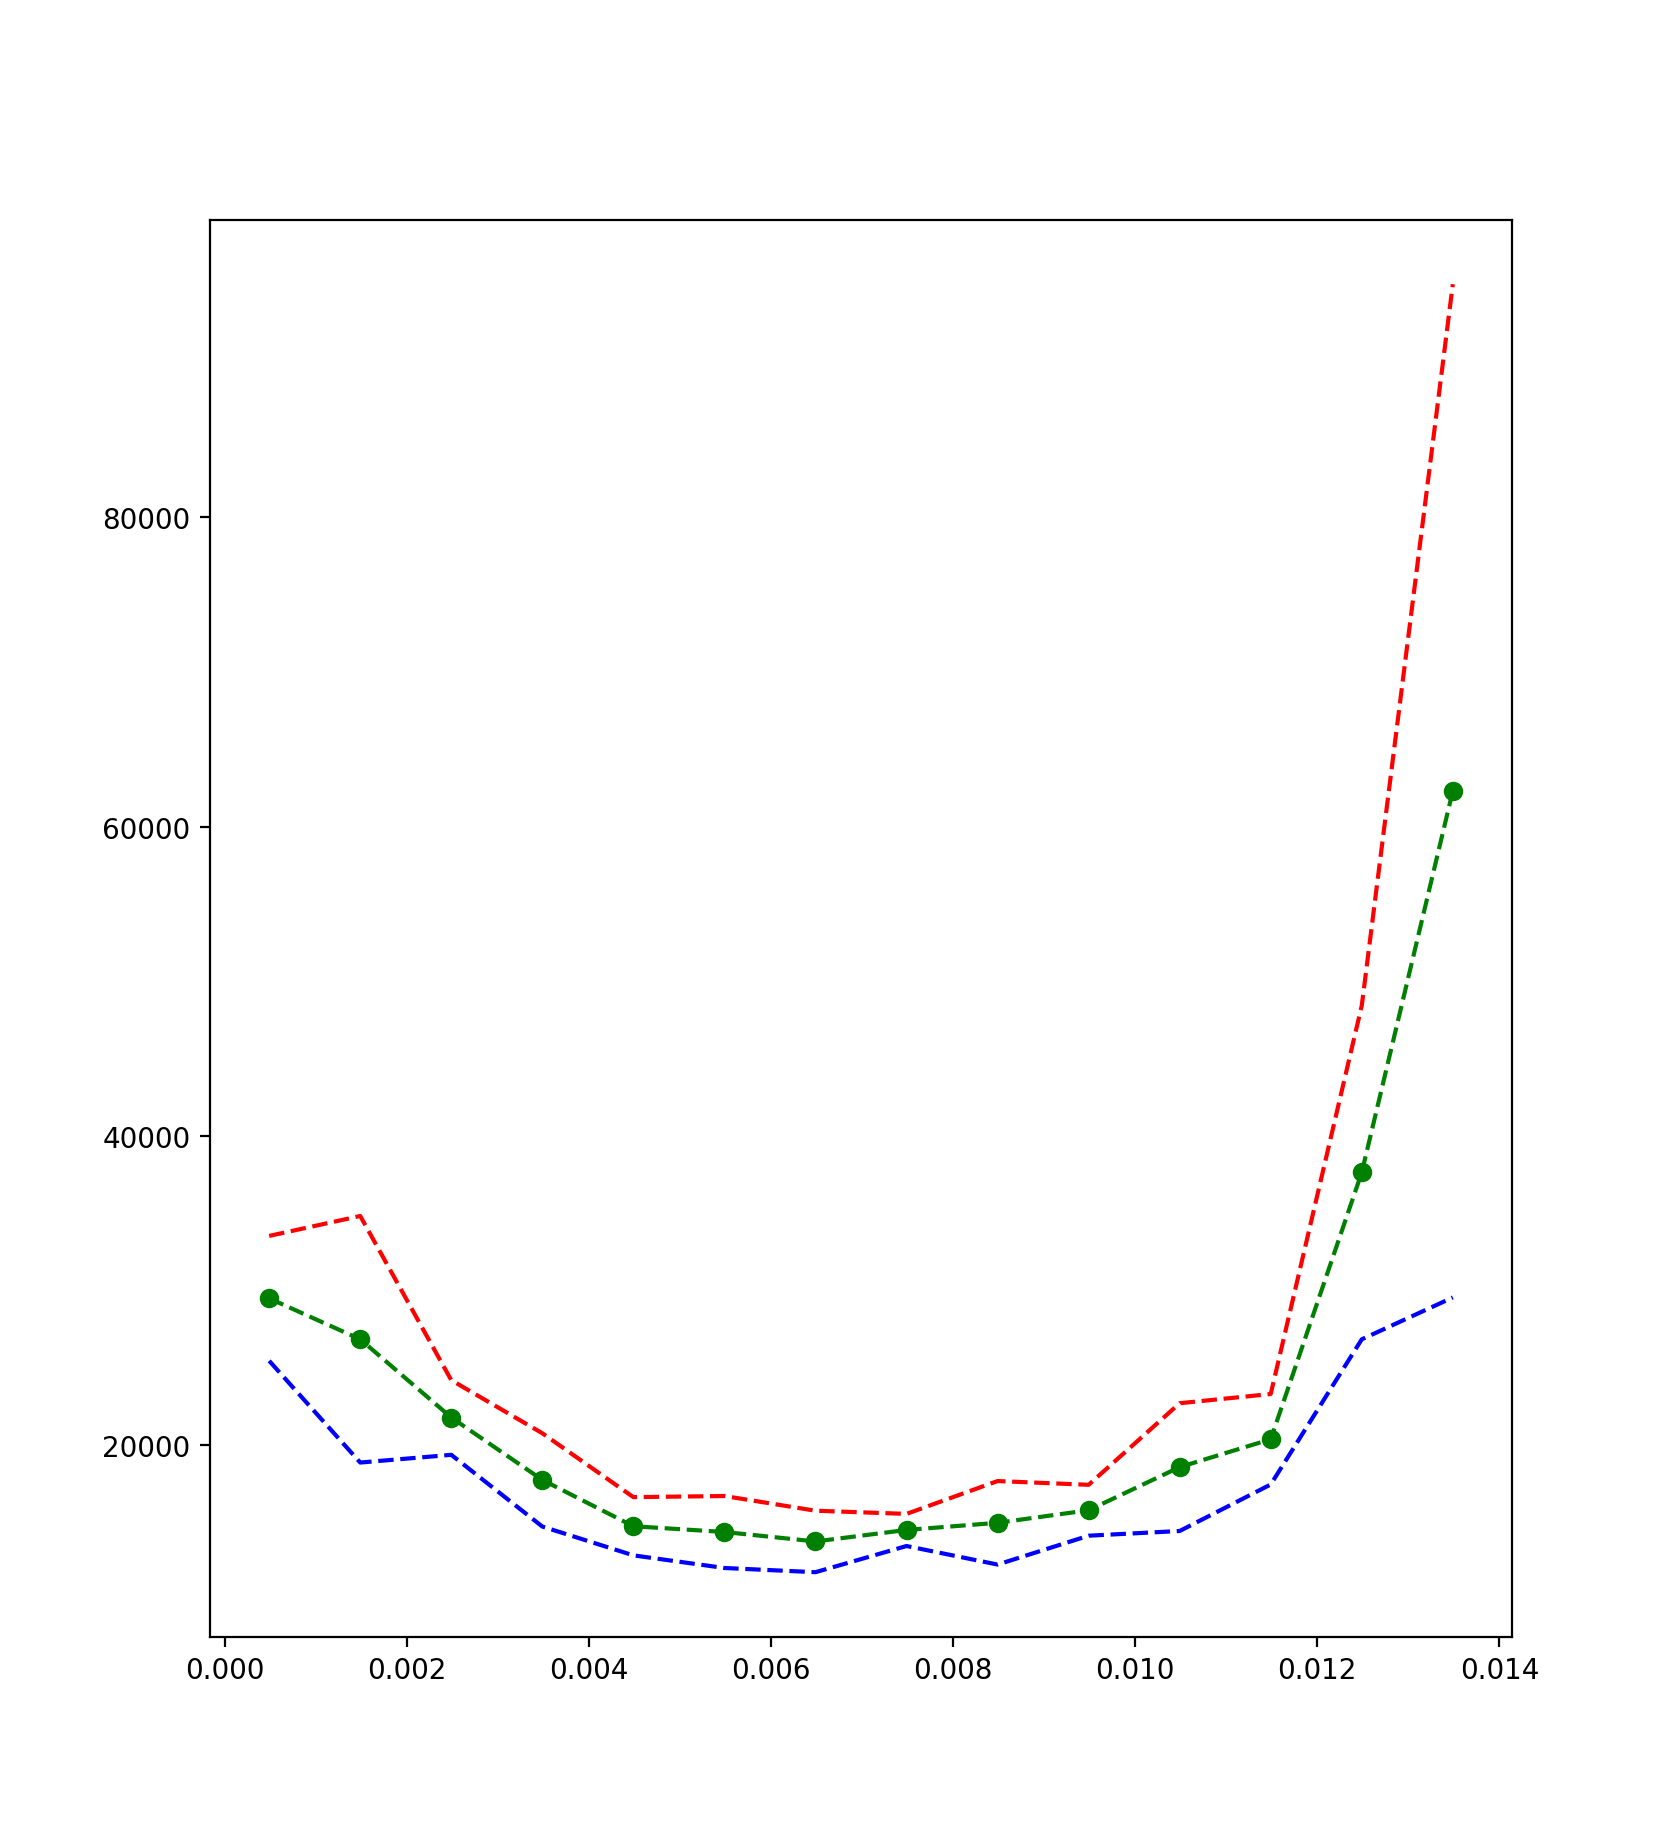
\includegraphics[width=0.8\linewidth]{imgs/ER_p_variation/n=1024 a=025.png}
      \caption*{$n=1024$}
      \label{fig:sub2}
    \end{subfigure}
\caption*{Sulle ascisse sono rappresentati i valori di $p$ mentre sulle ordinate i tempi di assorbimento. La curva in verde rappresenta il valore medio ricavato dai test, mentre le curve in blu e rosso descrivono i bound ottenuti rispettivamente sottraendo e sommando la deviazione standard al valore medio.}
\end{figure}
Dai grafici si evince come il minimo della funzione ottenuta non si trovi in $p=0$, come ci si poteva aspettare, per il quale il tempo di assorbimento \'e pari a $O(\frac{1}{\alpha}n\log{}n)$.
Questo implica l'esistenza di un valore di $p \geq 0$ per il quale il processo raggiunge lo stato di assorbimento in $o(\frac{1}{\alpha}n\log{}n)$ rounds con alta probabilit\'a.\\*
Dai dati ricavati nei diversi test eseguiti sugli Erd{\"o}s R\'enyi \'e possibile osservare che:
\begin{itemize}
    \item I valori ottenuti dalla prima serie di test descrivono un andamento decrescente del tempo di assorbimento almeno fino a $\frac{\log{n}}{n}$.
    \item La seconda serie di test descrive una crescita del tempo di assorbimento partendo da un punto di minimo non esplicitato, e prosegue fino al limite per $p$ fissato per questi test, che corrisponde a $\frac{3\log{n}}{2n}$.
\end{itemize}
Tutto ci\'o suggerisce come il punto di minimo $p_{min}$ si trovi in $[\frac{\log{n}}{n} , \frac{3\log{n}}{2n}]$.\\*
Sapendo che per il modello G($n$, $p$) il numero di archi in valore atteso \'e $\binom{n}{2}p$, se ne ricava che lo stato di assorbimento viene raggiunto pi\'u velocemente nei grafi che hanno un numero di archi E:
\begin{equation}
    \frac{(n-1)\log{n}}{2} \leq |E| \le1  \frac{3(n-1)\log{n}}{4}
\end{equation}
\end{document}